% !TEX encoding = UTF-8
% !TEX TS-program = pdflatex
% !TEX root = ../Tesi.tex
% !TEX spellcheck = it-IT

%************************************************

%************************************************
In questo capitolo si descriverà l'esecuzione della sperimentazione. Si partirà pertanto dai dati su cui quest'ultima è stata effettuata, proseguendo con la scelta delle modalità di esecuzione più interessanti e concludendo con una serie di tabelle e grafici contenenti i risultati ottenuti. 

\section{Decrizione del dataset}
Di seguito sono elencati i file che costituiscono il dataset. Gli esempi riportati di seguito sono stati ottenuti analizzando il sito del dipartimento di informatica di Urbana, IL: \texttt{www.cs.illinois.edu}

\subsubsection{urlsMap.txt}
Contiene la associazioni fra gli URL e il relativo codice identificativo. Questo è dovuto dalle ragioni spiegate in precedenza, ovvero ridurre i tempi di elaborazione e spazio di archiviazione. 
\\\\
\texttt{
http://cs.illinois.edu,3\\
http://cs.illinois.edu/prospective-students,4\\
http://cs.illinois.edu/current-students,5\\
http://cs.illinois.edu/courses,6\\
http://cs.illinois.edu/alumni,7\\
http://cs.illinois.edu/research,8\\
http://cs.illinois.edu/news,9\\
http://cs.illinois.edu/partners,10\\
http://cs.illinois.edu/about-us,11\\
. . .\\
}
\subsubsection{vertex.txt}
Contiene il contenuto testuale di ogni pagina esplorata. Ogni riga è quindi formata da il codice identificativo di un URL e il relativo contenuto.
\\\\
\texttt{
1	department of computer science at illinois engineering at ...\\
2	prospective students department of computer science at ...\\
3	current students department of computer science at ...\\
4	courses department of computer science at illinois ...\\
5	alumni department of computer science at illinois ...\\
6	research department of computer science at illinois    ...\\
7	news department of computer science illinois engineering ...\\
8	partners department of computer science at illinois ...\\
9	about us department of computer science at illinois ...\\
. . .\\
}
\subsubsection{edges.txt}
Questo è il file principale per la generazione delle sequenze, qui sono immagazzinate tutte le relazioni fra le pagine, ovvero gli archi che le collegano. 
\\\\
\texttt{
1	1\\
1	2\\
1	3\\
1	4\\
1	5\\
1	6\\
1	7\\
1	8\\
1	9\\
. . .\\
}
\subsubsection{sequencesIDs.txt}
Contiene le sequenze generate. I codici relativi alle pagine web sono separati da '' -1 '' e la linea finisce con un '' -2 ''. Da notare che sono riportate le sequenze che partono da un nodo casuale del grafo.
\\\\
\texttt{
137 -1 2 -1 27 -1 8 -1 52 -1 53 -1 8 -1 8 -1 10 -1 13 -1 -2\\
506 -1 5 -1 14 -1 11 -1 6 -1 2 -1 27 -1 114 -1 111 -1 11 -1 -2\\
424 -1 4 -1 12 -1 6 -1 8 -1 53 -1 4 -1 7 -1 12 -1 8 -1 -2\\
616 -1 5 -1 6 -1 8 -1 8 -1 9 -1 1 -1 21 -1 6 -1 3 -1 -2\\
51 -1 7 -1 7 -1 38 -1 38 -1 25 -1 103 -1 27 -1 113 -1 12 -1 -2\\
429 -1 10 -1 3 -1 6 -1 4 -1 11 -1 8 -1 9 -1 9 -1 3 -1 -2\\
783 -1 421 -1 5 -1 9 -1 7 -1 5 -1 2 -1 8 -1 2 -1 24 -1 -2\\
506 -1 5 -1 8 -1 52 -1 53 -1 25 -1 40 -1 13 -1 11 -1 13 -1 -2\\
638 -1 63 -1 153 -1 62 -1 63 -1 152 -1 63 -1 155 -1 13 -1 7 -1 -2\\
. . .\\
}
\subsubsection{sequencesIDsFromHomepage.txt}
Contiene le sequenze generate che partono da uno stesso nodo. La generazione di questo file avviene esplicitando il nodo di origine di ogni sequenza nella fase di generazione.
\\\\
\texttt{
1 -1 8 -1 2 -1 14 -1 2 -1 2 -1 10 -1 14 -1 66 -1 3 -1 -2\\
1 -1 18 -1 39 -1 8 -1 8 -1 24 -1 1 -1 4 -1 7 -1 25 -1 -2\\
1 -1 23 -1 -2\\
1 -1 16 -1 10 -1 3 -1 29 -1 29 -1 4 -1 25 -1 97 -1 108 -1 -2\\
1 -1 20 -1 20 -1 1 -1 11 -1 3 -1 2 -1 9 -1 10 -1 13 -1 -2\\
1 -1 25 -1 48 -1 48 -1 44 -1 42 -1 4 -1 7 -1 38 -1 38 -1 -2\\
1 -1 25 -1 115 -1 4 -1 11 -1 11 -1 1 -1 2 -1 26 -1 13 -1 -2\\
1 -1 24 -1 4 -1 9 -1 60 -1 56 -1 6 -1 25 -1 113 -1 116 -1 -2\\
1 -1 21 -1 25 -1 135 -1 32 -1 13 -1 4 -1 25 -1 149 -1 59 -1 -2\\
. . .\\
}

\section{Metodologie confrontate}
La sperimentazione si è svolta confrontando i risultati ottenuti attraverso l'applicazione di diversi algoritmi di clustering su dataset ottenuti da differenti rappresentazioni. In seguito verrano descritte le diverse rappresentazioni, i diversi algoritmi di clustering utilizzati e le metriche applicate per ottenere dei valori significativi alla valutazione.
\subsection{Partizionamento del Grafo Web}
Sono stati applicati metodologie derivanti dalla teoria dei grafi per l'estrazione di strutture connesse all'interno del grafo web. Questo può essere utile nella individuazione di comunità all'interno di grafi come ad esempio social network. La divisione del grafo in sotto-grafi può essere effettuata seguendo diversi approcci, inoltre il grafo costruito su di un normale sito web è caratterizzato solitamente da un numero elevato di collegamenti tra pagine che indirizzano all'utilizzo di alcune tipologie di partizionamento piuttosto che altre. Infatti misure come la betweenness (ovvero il valore dato ad un arco che rappresenta quante più volte questo è attraversato nel percorrere il cammino più breve fra due nodi qualsiasi) non hanno restituito risultati significativi.
\\
L'analisi del grafo considera unicamente le relazioni che intercorrono fra le pagine web e tralascia informazioni riguardanti il contenuto.
\begin{figure}[htb]
	\centering
	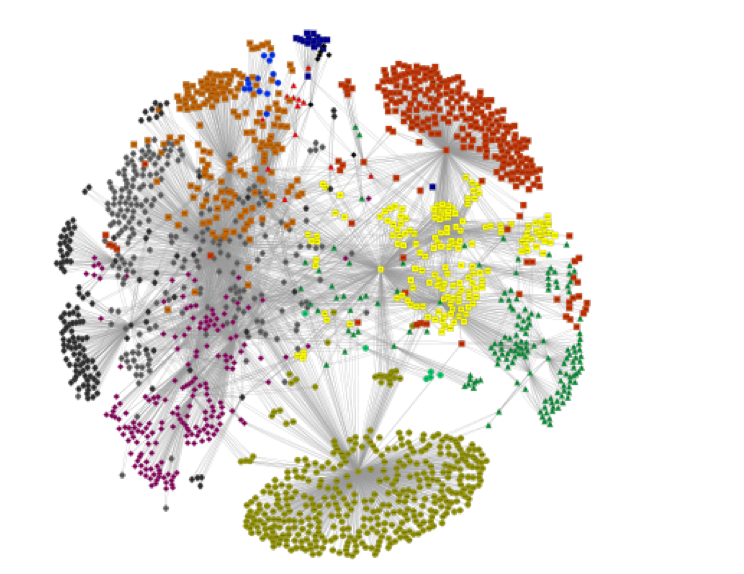
\includegraphics[width = 150mm]{graphpartitioning.png}
	\caption{Partizionamento di un grafo.}
	\label{modularity}
\end{figure}

\subsection{URL Embedding}
Considerando i random walk generati sul grafo come frasi, è possibile applicare algoritmi di word embedding per raggruppare le pagine sulla base del contesto in cui appaiono, ovvero le pagine che più verosimilmente appariranno insieme nelle sequenze di random walk. Anche questo approccio considera unicamente le relazioni fra le pagine, ma i percorsi casuali generati, considerati come frasi, raggruppano in cluster pagine che appariranno nello stesso random walk più volte, cosa che avverrà tanto più una pagina avrà collegamenti direzionati all'altra pagina. Apprendendo le rappresentazioni dai cammini invece che dal partizionamento del grafo si codificano le pagine in uno spazio vettoriale con i benefici che conseguono. La fase di URL embedding è stata effetuata l'algoritmo Word2vec.

\subsection{Text Mining}
Qui viene effettuata l'analisi testuale della pagina web, utilizzando tecniche derivanti dal Text Mining. I contenuti all'interno di uno stesso sito web avranno una struttura e termini comuni, differenziandosi al variare dell'argomento trattato. La struttura gerarchica di un sito web organizza solitamente le pagine in sezioni simili. Questa metodologia tuttavia, considera solo l'informazione testuale, assumendo che i termini all'interno del sito web siano indipendenti l'uno dall'altro (cosa che nei documenti che trattano argomenti specifici non  vero) così come i documenti, ignorando le relazioni interdipendenti tra questi. Il web si discosta dall'analisi classica dei documenti proprio per le relazioni che intercorrono tra le pagine, tuttavia l'analisi testuale rimane molto importante.
\\
Nella fase di sperimentazione è stata utilizzata una rappresentazione vettoriale della frequenza dei termini all'interno dell'insieme delle pagine web, calcolata con la tecnica della \textit{frequency–inverse document frequency} (tf-idf).

\subsection{Informazione combinata}
I risultati hanno evidenziato che l'analisi singola, sia della correlazione tra le pagine sia del contenuto testuale, non basta a codificare esaustivamente la conoscenza che una pagina web può offrire. Entrambe le informazioni sono rilevanti ed andrebbero processate combinatamente. Il vantaggio di associare le relazioni in uno spazio vettoriale offre il vantaggio usare la stessa rappresentazione e quindi di unire i vettori derivanti dagli algoritmi di word embedding con quelli derivanti dall'analisi di contenuto testuale. 
\\
Così facendo è possibile dare più importanza ad una tipologia di informazione piuttosto che ad un altra, andando a modificare il rapporto tra le dimensioni dei vettori.


\section{Algoritmi utilizzati}
Vengono riportati di seguito gli algoritmi di clustering testati sul dataset generato. L'obiettivo rimane comunque verificare se la soluzione proposta rappresenti un miglioramento ed un possibile alternativa alle soluzioni più usate e consolidate nell'ambito del clustering di pagine web.
\begin{itemize}
\item \textbf{WalkTrap}
È un approccio basato su Random Walk. L'idea generale è che se vengono generati dei Random Walk sul grafo, i percorsi rimarrano probabilmente all'interno della stessa comunità perchè ci sono meno archi che congiungono comunità diverse. 
\\
L'algoritmo esegue piccoli Random Walk (dipendente da un parametro in input) è usa i risultati per fondere comunità diverse in maniera bottom-up. Tagliando il dendrogramma risultante ad una certa altezza è possibile ricevere il numero di cluster desiderati.

\item \textbf{Fastgreedy}
È un approccio gerarchico bottom-up. Cerca di ottimizzare una funzione di modularità in maniera greedy, euristica attuata effettuando la scelta migliore con le informazioni in possesso ad ogni iterazione.
Inizialmente ogni nodo è una comunità separata e ricorsivamente si procede ad unire i nodi in modo che la fusione porti al massimo aumento di modularità rispetto al valore corrente. 
\\
L'algoritmo finisce quando non è più possibile aumentare la modularità. È un metodo veloce, solitamente usato come primo approccio perchè non ha parametri da modificare.
\item \textbf{K-Means}
Divide il dataset in un numero prefissato $k$ di cluster. Inizialmente vengono scelti casualmente $k$ punti, non necessariamente facenti parte del dataset, chiamati centroidi. Si procede assegnando ogni data point al centroide più vicino e ricalcolando il centroide sulla media aritmetica dei punti contiene. 
\\
Questo processo di assegnazione dei data point e ricalcolo dei centroidi continua fino a quando non avvengono più assegnazioni. I $k$ cluster risultanti saranno quelli restituiti. Anche questo algoritmo rappresenta spesso il punto di partenza nell'analisi di un dataset, in quanto molto spesso porta a buoni risultati ma ha come svantaggio il dover sapere a priori il numero di cluster desiderati.

\item \textbf{DBSCAN}
Deriva da \textit{Density-Based Spatial Clustering of Applications with Noise} è un algortimo basato sulla densità, connettendo regioni di punti con densità sufficientemente alta. Fondamentalmente, un punto $q$  è direttamente raggiungibile da un punto $p$ se non viene superata una data distanza $\epsilon$ e se $p$ è circondato da un numero sufficiente di punti, allora $p$ e $q$ possono essere considerati parti di un cluster. 
\\
Si può affermare che $q$ è density-reachable da $p$ se c'è una sequenza $p_1, p_2,  \ldots, p_n$ di punti con $p_1 = p$ e $p_n = q$ dove ogni $p_{i+1}$ è density-reachable direttamente da $p_i$. Da notare che la relazione density-reachable non è simmetrica (dato che $q$ potrebbe situarsi su una periferia del cluster, avendo un numero insufficiente di vicini per considerarlo un elemento genuino del cluster). Di conseguenza la nozione density-connected diventa: due punti $p$ e $q$ sono density-connected se c'è un punto $o$ tale che sia $o$ e $p$ che $o$ e $q$ sono density-reachable.
\\
Un cluster, che è un sotto-insieme dei punti del database, soddisfa due proprietà:

\textit{i)}Tutti i punti all'interno del cluster sono mutualmente density-connected.
\textit{ii)}Se un punto è density-connected a un altro punto del cluster, anch'esso è parte del cluster.

\item \textbf{HDBSCAN}
Deriva da \textit{Hierarchical Density-Based Spatial Clustering of Applications with Noise}~\cite{Campello15}. Applica DBSCAN variando il valore dell $\epsilon$ ed integra i risultati restituendo cluster che stabilizzano meglio tale valore.
\\
Questo permette ad HDBSCAN di trovare cluster con densità diversa, principale svantaggio di DBSCAN.
\end{itemize}

\section{Metriche}
Valutare le performance di un algoritmo di clustering non è banale come contare il numero di errori o calcolare metriche quali la precision e la recall di un lgoritmo di apprendimento supervisionato. In particolare metriche di valutazione non dovrebbero prendere in considerazione gli specifici valori delle label dei cluster ma piuttosto considerare se il raggruppamento in cluster generato dall'algortimo definisce una separazione dei dati similmente a quanto fornito nella \textit{ground truth}, ovvero il vero valore delle label, o soddisfare qualche assunzione come quella che i membri che appartangono allo stesso cluster sono più simili rispetto a quelli di cluster differenti, utilizzando una data funzione di similarità.

\begin{itemize}
\item \textbf{Homogeneity}
Nota la ground truth, questo valore rappresenta quanto ogni cluster sia omogeneo, ovvero che contiene solo membri di una classe.
\item \textbf{Completeness}
Note la ground truth, indica se tutti i membri di una sono stati assegnati allo stesso cluster
\item \textbf{V-Measure} rappresenta la media armonica fra l'\textit{homogeneity score} e il \textit{completeness score}.
\end{itemize}
Nelle metriche presentate $0.0$ rappresenta il valore peggiore, mentre $1.0$ il perfect score. Questi valori offrono una interpretazione intuitiva e può aiutare alla scoperta degli errori commessi nella assegnazione. Fra i vantaggi è degno di nota che nessuna assunzione viene fatta sulla struttura dei cluster, quindi possono essere utilizzate con algoritmi che identificano cluster di forma diversa.
\begin{itemize}
\item \textbf{Adjusted rand index}
Nota la ground truth, ovvero le classi reali, e le assegnazioni di un algritmo di apprendimento, viene calcolata una funzione che misura la similarità delle due informazioni, ignorandole permutazioni. I valori che può assumere vanno da $-1$ a $1$. Vicino allo $0$ rappresentano una assegnazione casuale delle etichette.
\\
Sia $C$ è gli assegnamenti della ground truth e $K$ le label predette, allora:
\\
$a$ è il numero di coppie di elementi che si trovano sia in $c$ che in $K$
\\
$b$ è il numero di coppie di elementi che si trovano in insiemi diversi in $C$ e in insiemi diversi in $K$.
Il \textbf{Random Index} è dato da:
\begin{equation}
RI = \frac{a + b}{C_2^n}
\end{equation}
Dove $C_2^n$ è il numero totale di tutte le possibili coppie nel dataset. 
\\
Il $RI$ non garantisce comunque che le assegnazioni casuali avranno valori prossimi allo $0$.
\\ Viene definito L'Adjusted Random Index:
\begin{equation}
ARI = \frac{RI - E[RI]}{\max (RI) - E[RI]}
\end{equation}
\item \textbf{Mutual Information}

\item \textbf{Silohuette}

\end{itemize}


\section{Risultati ottenuti}
tabellazze tabellazze tabellazze tabellazze tabellazze tabellazzetabellazze tabellazze tabellazze tabellazze tabellazze tabellazzetabellazze tabellazze tabellazze tabellazze tabellazze tabellazzetabellazze tabellazze tabellazze tabellazze tabellazze tabellazzetabellazze tabellazze tabellazze tabellazze tabellazze tabellazzetabellazze tabellazze tabellazze tabellazze tabellazze tabellazzetabellazze tabellazze tabellazze tabellazze tabellazze tabellazze



